% see - https://juliacon.github.io/proceedings-guide/author/

% JuliaCon proceedings template
\documentclass{juliacon}
\setcounter{page}{1}

\newcommand{\todo}[1]{\textcolor{red}{\textbf{TODO:} #1}}

\usepackage{hyperref}
\DeclareRobustCommand{\arch}[1]{\hyperlink{#1}{#1}}

\usepackage[normalem]{ulem}
\useunder{\uline}{\ul}{}

\usepackage{listings}
\usepackage{inconsolata}  % Monospaced font with bold support
\usepackage{multirow}
\usepackage{amsmath}

\definecolor{mBlue}{rgb}{0.39,0.39,1.0}
\definecolor{mRed}{rgb}{1.0,0.39,0.39}
\definecolor{mCyan}{rgb}{0.17,0.69,0.79}
\definecolor{mGreen}{rgb}{0.08,0.70,0.15}
\definecolor{mBrown}{rgb}{0.6,0.6,0.06}
\definecolor{lightpurple}{RGB}{150, 100, 200}

\lstdefinelanguage{Julia}{
    keywords={function, end, for, while, if, else, elseif, return, struct, mutable,
            abstract, type, using, import, export, const, let, do, try, catch,
            finally, macro, quote, module, baremodule, AbstractVector, Matrix, Float32},
    keywordstyle=\bfseries\color{mGreen},
    sensitive=true,
    comment=[l]\#,
    morestring=[b]",
    morestring=[b]',
    emph={[1]sqrt, println, push!, pop!, length, size, sum, mean, map, filter, reduce, rand},
    emphstyle={[1]\color{lightpurple}},
}

\begin{document}

% **************GENERATED FILE, DO NOT EDIT**************

\title{XK.jl: Composable and Portable Multi-GPU BLAS in Julia}

\author[1]{Romain PEREIRA}
\author[1]{Alexis MONTOISON}
\author[1]{Michel SCHANEN}
\author[1]{Swann PERARNAU}
\affil[1]{University}
\affil[2]{Argonne National Laboratory, Lemont, IL 60439, USA}

\keywords{Julia, BLAS, Macro-dataflow}

\hypersetup{
pdftitle = {XK.jl: Composable and Portable Multi-GPU BLAS in Julia},
pdfsubject = {JuliaCon 2022 Proceedings},
pdfauthor = {Romain PEREIRA, Alexis MONTOISON, Michel SCHANEN, Swann PERARNAU},
pdfkeywords = {Julia, BLAS, Macro-dataflow},
}



\maketitle

\begin{abstract}

% Romain to Alexis: you seem not to like 'An XKBlas program ...' -- this is my intent here, in the sense that an 'XKBlas program' has no clue of what happens outside these task-generating routines


This paper introduces XK.BLAS: the BLAS module of the Julia package XK.jl.
This module provides BLAS APIs that are portable across all three major GPU vendors (AMD, Intel, NVIDIA) for multi-device architectures.
XK.BLAS is built on top of the XKRT tasking runtime systems and the XKBlas library.
An XKBlas program is a sequence of task-generating routines with no explicit handling of memory (such as allocation and data movement) or scheduling decisions (such as target device selection).
Memory is instead lazily allocated, migrated, and evicted, while tasks are automatically distributed across available devices.
Tasks are composable, so that fine-grained dependencies are inferred from the memory regions they access, allowing concurrent data movement and kernel execution across different routines when the dataflow permits.
We evaluate primitives of XK.BLAS and its use as a multi-GPU backend for the package Krylov.jl.
We show up to 2.8× speedup when scaling from 1 to 4 H100 GPUs.
More importantly, XK.BLAS enables solving problems that would not otherwise fit on a single GPU, with no code changes at all.

\end{abstract}

%%%%%%%%%%%%%%%%%%%%%%%%%%%%%%%%%%%%%%%%%%%%%%%%%%%%%
\section{Introduction}
%%%%%%%%%%%%%%%%%%%%%%%%%%%%%%%%%%%%%%%%%%%%%%%%%%%%%

% CONTEXT - BLAS and Julia
The Basic Linear Algebra Subprograms (BLAS~\cite{blas-spec}) specify routines for scientific computing.
Original implementation (Netlib, OpenBLAS) target CPUs.
GPU companies (AMD, Intel, NVIDIA) provide high-performance implementation (rocBLAS~\cite{rocblas}, OneMKL~\cite{onemkl}, cuBLAS~\cite{cublas}) for GPUs.
These libraries are fundamental building blocks for developing scientific software such as iterative solvers~\cite{montoison-orban-2023,AlMouhamed2023SpMV}.
However, despite the advent of multi-GPU servers, vendors' implementation only targets single-GPU: programmers are responsible for manually parallelizing execution across multiple devices (i.e., moving memory and synchronizing kernel executions).

% CONTEXT - BLAS and multi-GPU
This motivated the design of new multi-GPU BLAS implementation~\cite{BLASX, XKBlas, cublasXT, Chameleon, parsec24, MAGMA24, SLATE, PARALIA} that automates parallel execution from a sequential program that preserves historical BLAS APIs.
They are all implemented in C/C++ and tile routines~\cite{tile-blas} to distribute tasks to multiple devices.
Among these libraries, XKBlas~\cite{XKBlas} uniquely provides highly composable tasking interfaces with relaxed synchronizations between routines~\footnote{\url{https://gitlab.inria.fr/xkblas/dev/tree/v2.0}}.
It has shown great success in accelerating the sparse solver MUMPS~\cite{mumps} to multiple GPUs with only a few lines of code changes ($\simeq 10-20 \; LoC$) with great performance portability thanks to its underlying tasking model.

% PROBLEM - no multi-GPU BLAS in Julia
The Julia linear algebra ecosystem currently lacks similar libraries to automatically move memory and schedule BLAS routines on multi-device architectures.
Current practices involve manually moving memory and distributing work via vendor-specific libraries (AMDGPU.jl, CUDA.jl, oneAPI.jl), and dispatching linear algebra primitives depending on input data types (\texttt{ROCArray}, \texttt{CuArray}, \texttt{oneArray}).
A promising ongoing effort is cuNumeric.jl~\cite{krasowska2025reducing}, inspired by cuPyNumeric and built on top of Legion~\cite{legion}.
However, it is currently restricted to NVIDIA GPUs and remains at an early stage of development.

% Objective
This paper fills that gap in the Julia ecosystem by introducing the BLAS module of XK.jl (XK.BLAS): a package built on top of XKRT and XKBlas automating data motions and execution of BLAS across multi-device architectures.
% Contributions
Our contributions are the following:
\begin{itemize}
    \item[$\bullet$] The introduction of XK.BLAS provides composable and portable multi-GPU BLAS in Julia.
    \item[$\bullet$] Extensions to XKBlas to support BLAS 1 and 2 routines, that can be used as drop-in replacements in CPU programs (i.e., automatic multi-GPU parallelization with no code change at all).
    \item[$\bullet$] The implementation of a new backend for Krylov.jl~\cite{montoison-orban-2023}, a collection of Krylov solver, using XK.BLAS to provide performant and portable parallelization on most of its solvers across multi-GPU architectures.
\end{itemize}
The paper is organized as follows.  
Section~\ref{sec:background} introduces the background of XK.BLAS.  
Section~\ref{sec:impl} presents its implementation and the extensions enabling improved support for Krylov solvers.
Section~\ref{sec:eval} evaluates XK.BLAS primitives and their integration as a multi-GPU backend for Krylov.jl.  
Section~\ref{sec:conclusion} concludes the paper.

%%%%%%%%%%%%%%%%%%%%%%%%%%%%%%%%%%%%%%%%%%%%%%%%%%%%%
\section{Background} \label{sec:background}
%%%%%%%%%%%%%%%%%%%%%%%%%%%%%%%%%%%%%%%%%%%%%%%%%%%%%


\begin{figure*}[]
    \centering
    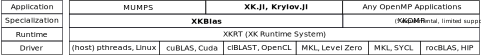
\includegraphics[width=\linewidth]{figures/software-stack.pdf}
    \caption{An Overview of the XK.jl software stack}
    \label{fig:xkblas-software-stack}
\end{figure*}

XK.jl is a Julia framework for composable and portable multi-GPU linear algebra.  
Its core module, XK.BLAS enables sequential CPU-like code to run efficiently across multiple GPUs by automatically managing memory, scheduling tasks, and overlapping computation and communication.  
We first introduce Krylov.jl as a motivating application, and discuss how its reliance on BLAS routines motivates the extensions and multi-device capabilities of XK.BLAS.

%----------------------------%
\subsection{Krylov.jl} \label{sec:krylov}
%----------------------------%

The package Krylov.jl implements over 35 Krylov methods for solving a variety of problems, including square linear systems, least-squares problems, least-norm problems, and structured $2 \times 2$ block systems.
It is the primary motivation for the BLAS module of XK.jl.  
Krylov.jl specifies a set of routines that need to be implemented to execute its solvers agnostically across devices.  
On the CPU, Krylov.jl dispatches these routines through Libblastrampoline (LBT), allowing seamless switching between different BLAS backends such as Intel MKL, AOCL, Apple Accelerate, or BLIS.  
On GPUs, multiple dispatch is used based on the type of the GPU vector (like \texttt{CuVector} or \texttt{ROCVector}) to target the appropriate GPU BLAS implementation.  
% It is also possible to extend Krylov.jl with custom methods for user-defined types.  

Solvers are implemented as if they were executing on a single CPU, with no considerations on memory locality, nor expressing any parallelism explicitly.
We illustrate it on code~\ref{lst:krylov-example} with a few lines of code extracted from its implementation of the conjugate gradient method.
Line~3 runs the operator \texttt{kmul!} between the variables $A$ and $p$ and stores the result in the variable $Ap$.
For instance, if $Ap$, $A$, and $p$ respectively are \texttt{CuVector}, \texttt{CuMatrix}, and \texttt{CuVector}, then Krylov.jl dispatches to the \texttt{gemv} implementation of cuBLAS assuming the memory is already present and coherent on the device.
The executing thread waits for the operator completion, and then on line 2, it computes the dot product and stores the real part of the results to the variable \texttt{pAp} in the host memory.
Line 4, it computes $\alpha = \gamma / pAp$ on the host.

\lstset{xleftmargin=2em}
\begin{lstlisting}[
    float,
    floatplacement=tbp,
    language = Julia,
    numbers=left, 
    label={lst:krylov-example},
    caption={A few lines of code from Krylov.jl implementation of the conjugate gradient method.}
]
function cg(A, b; kwargs...)
    # [...]
    kmul!(Ap, A, p)       # Ap  := A * p
    pAp = kdotr(n, p, Ap) # pAp := real(p'Ap)
    # [...]
    α = γ / pAp
    # [...]
end
\end{lstlisting}

Currently, GPU support relies on GPUArrays.jl and its AMDGPU.jl, CUDA.jl, and oneAPI.jl specializations.  
Programmers must explicitly and synchronously move memory from the host to the device before solver execution by declaring \texttt{ROCArray}, \texttt{CuArray}, or \texttt{oneArray} data structures.
The Krylov.jl backend then dispatches to the respective vendor-specific single-GPU BLAS libraries using Julia's multiple dispatch feature.  
The primary motivation of this work is to provide multi-GPU support for Krylov.jl solvers without modifying its existing 12,000 lines of code, which implement the Krylov solvers.
All methods heavily rely on BLAS 1 and 2 routines, while two of them, the block Krylov methods block-MINRES and block-GMRES, also use LAPACK and BLAS 3 routines.
These remain as future work.
% None of them currently require vectors and matrices to be written-back onto the host memory.
% However, they do require scalar results of BLAS 1 (such as the \texttt{dot} line 4 of Code~\cite{lst:krylov-example}) to be written-back.


%----------------------------%
\subsection{XKBlas, XKRT}
%----------------------------%

\lstset{xleftmargin=2em}
\begin{lstlisting}[
    float,
    floatplacement=tbp,
    language = Julia,
    numbers=left, 
    label={lst:xkblas-example},
    caption={Pseudo-code of an XKBlas program. The \texttt{trsm\_async} and \texttt{gemm\_async} spawn tasks executing the routine on submatrices, that synchronizes depending on sequential data dependencies. The \texttt{memory\_host\_coherent\_async} spawns a task that writes-back the passed memory region (i.e., the matrix C) to its original host replica.}
]
# A, B and C are matrices on the host memory
# Routines are executed on available devices

# trsm reads A, B and writes B
trsm_async(A, B,    tile_size=n/2);

# gemm reads A, B, C and writes C
gemm_async(A, B, C, tile_size=n/2);

 # ask for host write-back
memory_host_coherent_async(C);

# wait for the completion of previous tasks
sync();

# At this point of the execution, the matrix
# - C was written-back to the host memory.
# - B was not.
\end{lstlisting}

\begin{figure}[]
    \centering
    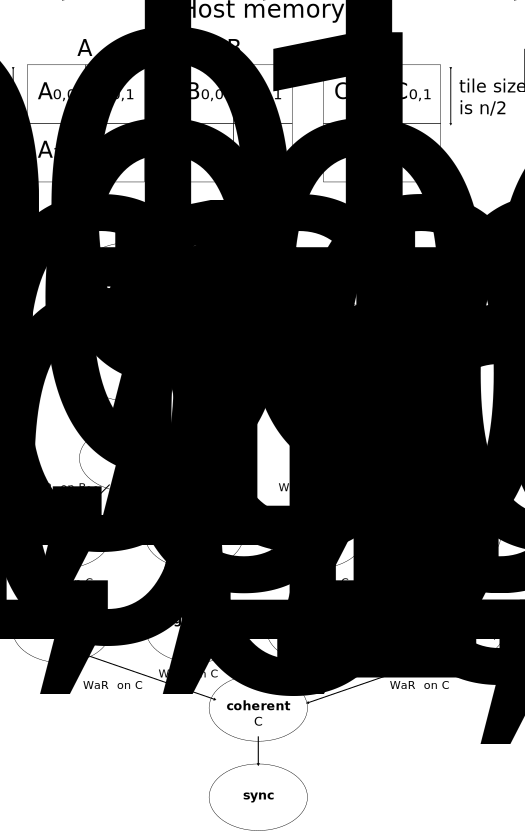
\includegraphics[width=0.75\linewidth]{figures/xkblas/trsm-gemm.pdf}
    \caption{Task graph resulting from the XKBlas sequence on Code~\ref{lst:xkblas-example}. Tasks and their associated  memory are distributed to available GPUs in parallel, and concurrently to the graph creation. Minimal data motions are ensured from conflicting memory accesses by the XKRT internal coherence protocol.}
    \label{fig:xkblas-trsm-gemm}
\end{figure}

The XKBlas library~\cite{XKBlas} accelerates BLAS 3 in the MUMPS linear solver~\cite{mumps} on multi-GPU architectures.
This work shares the same original motivations: accelerate a sequential host program to multiple devices.
It was originally built on top of the Kaapi tasking runtime system~\cite{kaapi} and had been recently (2024-2025) rewritten on top of the XKRT runtime system~\footnote{\url{https://github.com/rpereira-dev/xkrt}}---a fork of Kaapi that supports byte-granular data dependencies and motion for macro-dataflow tasks ala Legion~\cite{legion}.
We summarize the software stack in Figure~\ref{fig:xkblas-software-stack}.
The key aspects of XKBlas are:
\begin{itemize}
    \item[$\bullet$] (1) Automated memory management. XKBlas APIs use host memory pointers and lazily replicates on the executing devices' memories. XKBlas book-keeps memory coherence over routine invocations, so that the memory is assumed \emph{coherent} (aka. valid) only on the device that lastly wrote it.
    \item[$\bullet$] (2) Multi-GPU support. XKBlas internally tiles and distributes BLAS routines to available devices.
    \item[$\bullet$] (3) Asynchrony. XKBlas overlaps GPU kernel execution with data motion implicitly while ensuring a partial and correct parallel order of execution following the sequential program data dependencies that are well-defined by the BLAS specification: for instance, \texttt{gemm(A, B, C)} reads A, B, and C, and writes C.
\end{itemize}

An XKBlas task includes a kernel and a declaration of its memory accesses (read, write, and the host virtual memory region) so that a correct parallel order of execution can be deduced from data hazards (read-after-write, etc., on intersecting regions of memory) by its underlying runtime system.
An XKBlas program is a sequence of CPU-like routines spawning tasks that compose automatically to overlap independent data motion and computation---as illustrated on Code~\ref{lst:xkblas-example}.
The routines (\texttt{gemm\_async}) lines 3 and 4 spawn tasks to be executed and return before their completion.
The \texttt{sync} line 5 waits for the completion of all tasks previously spawned.
The \texttt{memory\_coherent\_async} line 11 spawns an empty task on the host to write-back the matrix D so the host memory is coherent by the completion of the \texttt{sync} line 12.
We illustrate the resulting task dependency graph in Figure~\ref{fig:xkblas-trsm-gemm}: independent tasks can execute in parallel on different GPUs.

XKBlas originally only supported BLAS 3 routines that represented the largest potential for GPU acceleration in MUMPS.
This paper extends it with support for the BLAS 1 and 2 routines to provide a multi-GPU backend to Krylov.jl.
%  and also provides a kernel language to implement custom routines natively in Julia.

% It also required a few line of code modifications to insert device-to-host data motion (\texttt{memory\_coherent\_async}) and synchronizations points (\texttt{sync}).

% %----------------------------%
% \subsection{LLVM, Julia}
% %----------------------------%
% \todo{Talk about LLVM and its compiler that can target SPIRV and NVPTX? or later maybe}



% TODO
% This paper introduces XKBlas.jl: a Julia programming environment for portable linear algebra workloads across multi-GPU systems built on top of XKRT.
% Using GPUCompiler.jl, XKBlas.jl provides its own enriched kernel language for implementing custom kernels, that portably executes across GPU architectures, and composes automatically with built-in BLAS routines thanks to dataflow dependencies detection.
% We illustrate XKBlas.jl sing it as a back-end for the Krylov.jl library.

% XKBlas.jl extends XKBlas with support for custom routines written in Julia via that composes automatically thanks to its underlying macro-dataflow programming model.

% XKBlas.jl is built on top of the dataflow runtime system XKRT.
% XKRT allows the automatic parallelization of CPU-alike computation, interpreting the host virtual memory as a shared memory space across devices, 
% Thanks to XKRT dataflow programming model, XKBlas.jl allows the programming of multi-GPU 
% XKBlas.jl extends XKBlas with support for custom routines written in Julia via that composes automatically thanks to its underlying macro-dataflow programming model.
% ---using Julia as an highly productive kernel languages and the XKBlas library as a high-performance parallelism orchestrator.


%%%%%%%%%%%%%%%%%%%%%%%%%%%%%%%%%%%%%%%%%%%%%%%%%%%%%
\section{XK.BLAS: multi-devices BLAS in Julia} \label{sec:impl}
%%%%%%%%%%%%%%%%%%%%%%%%%%%%%%%%%%%%%%%%%%%%%%%%%%%%%

XK.BLAS provides the core multi-device BLAS functionality of XK.jl.  
In this section, we present its architecture and runtime (XKRT), the available execution model flavors, and our extensions to support BLAS 1 and 2 routines.  
We also show how XK.BLAS can serve as a drop-in multi-GPU backend for Krylov.jl, enabling efficient execution without modifying its original CPU-based source code.

\begin{lstlisting}[
    float,
    floatplacement=tbp,
    language = Julia, 
    numbers=left, 
    label={lst:julia-xkblas-example},
    caption={An XK.BLAS program example.}
]
using LinearAlgebra, Random, XK

# Run parameters
const T = Float32
m = n = k = 16_384
lda, ldb, ldc = m, k, m
alpha = T(1.0)
beta = T(0.0)
transA = transB = XK.BLAS.NO_TRANS

# Create host matrices
A = Matrix{T}(undef, m, k)
B = Matrix{T}(undef, k, n)
C = Matrix{T}(undef, m, n)

# Execution on all available devices - 3 flavors:

# (F1) Blocking, and automatic write-back
XK.BLAS.gemm(
    transA, transB,
    alpha, A, B,
    beta,  C
)

# (F2) Blocking, no automatic write-back
XK.BLAS.gemm_sync(
    transA, transB,
    alpha, A, B,
    beta,  C
)

# (F3) Non-blocking, no automatic write-back
XK.BLAS.gemm_async(
    transA, transB,
    alpha, A, B,
    beta,  C
)
XK.BLAS.sync()
\end{lstlisting}

%----------------------------%
\subsection{Binding to a C/C++ library}
%----------------------------%

XKBlas and XKRT are C++ libraries that expose a C API.  
XK.jl automatically generates bindings to these C APIs using Foreign Function Interfaces (FFIs) generated via Clang.jl.  
On top of these bindings, we manually implement wrappers that provide idiomatic Julia interfaces, allowing seamless integration within the Julia linear algebra programming environment, as illustrated in Code~\ref{lst:julia-xkblas-example}.  
For example, XK.BLAS dispatches routines to the corresponding XKBlas implementation based on parameter precision (\texttt{Float32} maps to single, \texttt{Float64} to double, etc.).  
Additionally, its BLAS routines and the \texttt{memory\_coherent\_async} API support native Julia linear algebra types such as \texttt{AbstractVector} and \texttt{AbstractMatrix}, as shown on line 19.

%----------------------------%
\subsection{Execution model flavors}
%----------------------------%

Additionally, XK.BLAS provides three execution model flavors.  
The input objects always reside in host memory, but each flavor defines how synchronization and write-back are handled:

\begin{itemize}
    \item[$\bullet$] (F1) Drop-in (line 19). The calling thread blocks until all tasks complete, and every byte written on any device is automatically written back to the host. In the code example, the executing threads wait for the \texttt{gemm} tasks to finish, and the matrix \texttt{C} is implicitly updated on the host.
    
    \item[$\bullet$] (F2) Synchronous (line 25). The calling thread blocks until all tasks complete, but there is no automatic write-back. Programmers can explicitly request write-back via \texttt{XK.BLAS.memory\_host\_coherent\_async}. In the code example, the threads wait for the \texttt{gemm} tasks, but parts of \texttt{C} remain on the devices until explicitly synchronized.
    
    \item[$\bullet$] (F3) Asynchronous (line 33). The calling thread only spawns tasks and returns immediately, without waiting for their completion. Programmers can enforce completion by calling \texttt{XK.BLAS.sync()}. As in (F2), there is no automatic write-back. In the example, the tasks are spawned, the function returns, and completion is enforced later via \texttt{sync()}.
\end{itemize}

Originally, XKBlas only supported flavor (F3). We extended it with (F1) and (F2) to serve as drop-in replacements for CPU BLAS programs, requiring no changes to existing code.

%----------------------------%
\subsection{Support for BLAS 1 and 2} \label{sec:blas1-2}
%----------------------------%

\begin{figure}[]
    \centering
    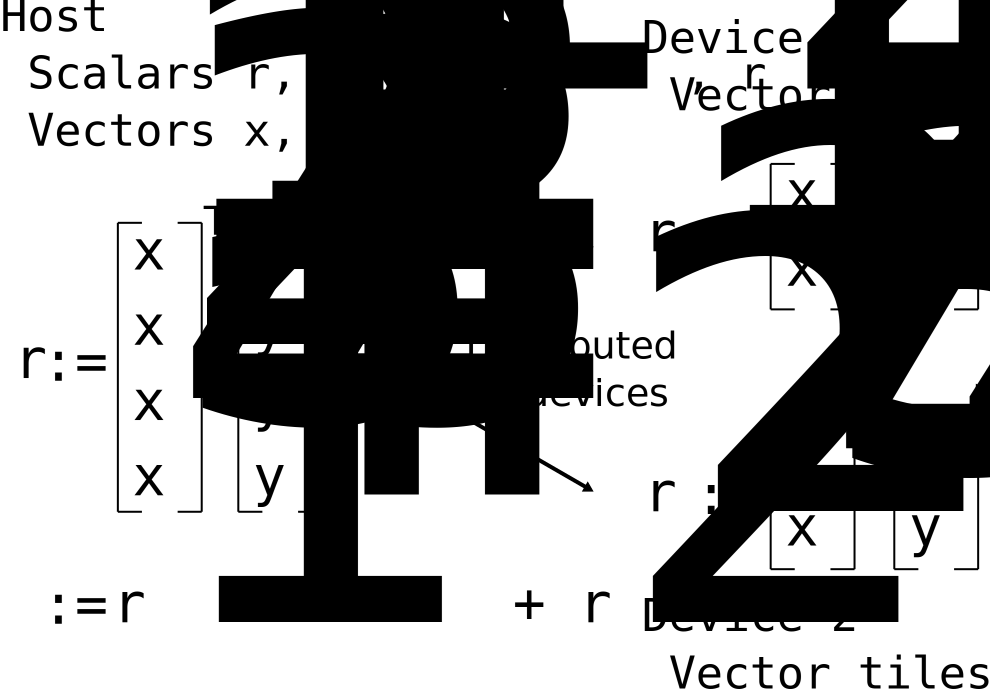
\includegraphics[width=0.7\linewidth]{figures/xkblas/dot.pdf}
    \caption{\texttt{dot} distributed from the host to two devices with one tile per device.}
    \label{fig:xkblas-dot}
\end{figure}

\begin{figure*}[]
    \centering
    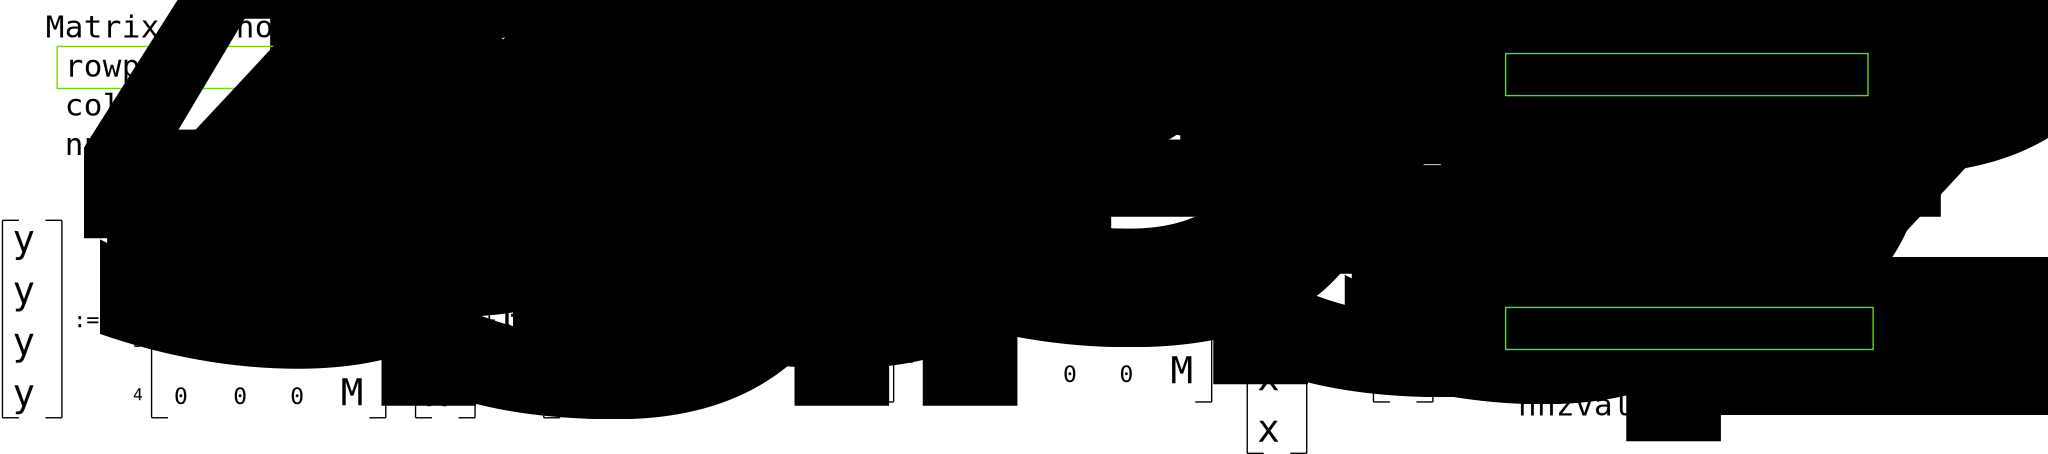
\includegraphics[width=0.95\linewidth]{figures/xkblas/spmv.pdf}
    \caption{\texttt{spmv} for CSR matrices distributed from the host to two devices with one tile per device.}
    \label{fig:xkblas-spmv}
\end{figure*}

% \todo{explain here or earlier that BLAS original CPU API use (M, m, n, LD)}
% AM: Romain, je comprends ce que tu veux expliquer exactement avec ton todo au dessus.
% \emph{Support for BLAS 1 and BLAS 2.}

The Krylov.jl library relies extensively on BLAS 1 and 2 routines (\texttt{axpby}, \texttt{dot}, \texttt{nrm2}) and matrix vector operations (\texttt{gemv}, \texttt{spmv}).  
These routines were not originally supported in XKBlas.
We therefore implemented them, and present our approach in this section.

As with the original BLAS 3 routines, BLAS 1 and 2 operations are tiled into tasks and distributed across multiple devices.
Each task eventually launches a vendor-specific kernel (cuBLAS, hipBLAS, or oneMKL) on a subvector or submatrix.  
XKBlas tiles dense matrices and vectors contiguously using a fixed tile size, improving memory locality on devices when chaining multiple kernels.
Figures~\ref{fig:xkblas-dot} and~\ref{fig:xkblas-spmv} illustrate our multi-device implementations of \texttt{dot} and \texttt{spmv}.  

Currently, \texttt{spmv} only supports the Compressed Sparse Row (CSR) format.
Given a sparse matrix of size $(m,n)$, our implementation preprocesses the matrix in four steps:
\begin{itemize}
    \item[$\bullet$] $\mathcal{S}_1$--Tile the matrix into blocks of size $(m_t \le m, n)$ and assign each block to a device,
    \item[$\bullet$] $\mathcal{S}_2$--Execute a custom kernel to adjust row indices for each tile so they are valid on the local device memory,
    \item[$\bullet$] $\mathcal{S}_3$--Compute the minimum and maximum column indices containing non-zero elements for each tile.
    \item[$\bullet$] $\mathcal{S}_4$--Run vendor specific preprocessing routines (\texttt{cusparseSpMV\_preprocess}, etc.).
\end{itemize}
The step $\mathcal{S}_3$ is optional.
If $\mathcal{S}_3$ is disabled, the entire vector $x$ will be moved on the executing device.
For instance on Figure~\ref{fig:xkblas-spmv}, all $x_1$, $x_2$, $x_3$ and $x_4$ will be copied to the device 2 even though only $x_3$ and $x_4$ are needed, since the matrix columns 1 and 2 are only zeroes.
However, if $\mathcal{S}_3$ is enabled, the runtime will only copy the smallest sub-vector that includes all lines with non-zeroes columns in the matrix---e.g., on the figure, only $x_3$ and $x_4$ are copied---which reduces data movements.
Such technique is used by the HPCG benchmark that uses a 7-diagonal matrix distributed with MPI~\cite{hpcg}.


All steps are performed only the first time the matrix is encountered, and the results are cached for later reuse.
% This is a well-known optimization for sparse matrices~\cite{} \todo{add reference}.  
Programmers can explicitly invalidate these caches if the matrix values change.

%----------------------------%
\subsection{A Multi-GPU Backend for Krylov.jl}
%----------------------------%

XK.jl introduces several new Julia types, namely \texttt{XKVector}, \texttt{XKMatrix}, and \texttt{XKSparseMatrixCSR}, which act as wrappers around specialized data structures while preserving existing CPU and GPU support through multiple dispatch.  
These types enable the integration of XK.jl with Krylov.jl without modifying its original programming model.

The XK.BLAS module overloads the default Krylov.jl backend by providing implementations based on the flavor (F2) API.  
This flavor ensures minimal data movement and remains fully compatible with Krylov.jl’s execution semantics (see Section~\ref{sec:krylov}).

For instance, adopting flavor (F3) would result in an incorrect execution order in Code~\ref{lst:krylov-example}.  
Specifically, the computation of $\alpha = \gamma / pAp$ (line~6) could be executed before the completion of the \texttt{kdotr} operation (line~4).  
Guaranteeing correct behavior in this case would require modifying Krylov.jl to introduce explicit synchronization points, which we intentionally avoid.

Conversely, flavor (F1) preserves correctness but incurs significant overhead due to frequent host-to-device (H2D) and device-to-host (D2H) memory transfers between solver iterations.  
By leveraging flavor (F2), XK.BLAS relies on XKRT’s internal memory coherence mechanisms to enforce correct execution order while minimizing data movement.

% \emph{Synchronous Execution Model}
% - \todo{say that there is not much overlap anyway between operations in iterative solvers - \cite{pereira23}}

% - XKBlas originally provides two execution model
%     - async = no automatic cache invalidation, no automatic write-back, task-spawning, returning before completion
%     - dropin = cache-invalidation, task-spawning, writes-back, returning after completion

% - Problem:
%     - async = require code modifications---
%     - sync = no automatic cache invalidation, no write-back, task-spawning, returning after completion


% %----------------------------%
% \subsection{Support for Custom Routines Natively in Julia}
% %----------------------------%
% \todo{leverage embbeded LLVM compiler to create custom routines natively in Julia --- ala OpenMP target regions}

% %----------------------------%
% \subsection{Composing Multiple Routines}
% %----------------------------%

% \todo{illustrate composability+}

%%%%%%%%%%%%%%%%%%%%%%%%%%%%%%%%%%%%%%%%%%%%%%%%%%%%%
\section{Evaluation} \label{sec:eval}
%%%%%%%%%%%%%%%%%%%%%%%%%%%%%%%%%%%%%%%%%%%%%%%%%%%%%

% %----------------------------%
% \subsection{Environments}
% %----------------------------%

We evaluate the performance of XK.BLAS using Julia v1.11.8 on the experimental environments shown in Table~\ref {tab:hardware}.
First, we evaluate a few of its routines to ensure proper binding between Julia and the underlying C/C++ runtime system, and scalability against the number of GPUs.
Then, we evaluate XK.BLAS as a multi-GPU backend for Krylov.jl.

% On the \arch{AMD-JLSE} architecture, there is a total of 4 PCI 4.0 (28GB/s) with 2 GPUs per bus.
% \todo{explain links topology? amd gpus topology is kinda complicated}
%           Inter-Device Numa Distance
%           D/D       0         1         2         3         4         5         6         7         8         9         
%           0         0         32        20        20        20        20        52        52        52        52        
%           1         32        0         52        52        52        52        20        20        20        20        
%           2         20        52        0         15        15        30        30        30        15        30        
%           3         20        52        15        0         30        15        30        15        30        45        
%           4         20        52        15        30        0         15        15        30        30        30        
%           5         20        52        30        15        15        0         30        45        30        15        
%           6         52        20        30        30        15        30        0         15        15        30        
%           7         52        20        30        15        30        45        15        0         30        15        
%           8         52        20        15        30        30        30        15        30        0         15        
%           9         52        20        30        45        30        15        30        15        15        0  

\begin{table}[h]
\centering
\caption{Hardware and software stack used in the evaluations}
\label{tab:hardware}
\resizebox{\columnwidth}{!}{%
\begin{tabular}{|l|c|c|c|}
\hline
\textbf{Name} & \textbf{Hardware (CPU)} & \textbf{Hardware (GPU)} & \textbf{Software} \\ \hline
\hypertarget{AMD-JLSE}{AMD-JLSE} & \begin{tabular}[c]{@{}c@{}}2x AMD EPYC\\ 7713 @2.0GHz\end{tabular} & 8x MI250X & \begin{tabular}[c]{@{}c@{}}rocm 6.3.2,\\ LLVM 19.1.0\end{tabular} \\ \hline
\hypertarget{NV2-JLSE}{NV-JLSE} & \begin{tabular}[c]{@{}c@{}}2x Intel(R) Xeon(R)\\ Platinum 8468 @3.8GHz\end{tabular} & 4x H100 & \begin{tabular}[c]{@{}c@{}}nvhpc 24.1,\\ LLVM 21.x\end{tabular} \\ \hline
\hypertarget{Aurora}{Aurora} & \begin{tabular}[c]{@{}c@{}}2x Intel Xeon CPU Max \\ Series (SPR) @2.0 GHz\end{tabular} & 6x PVC & oneapi 24.347.0 \\ \hline
\end{tabular}%
}
\end{table}
%----------------------------%
\subsection{Routines Benchmarking}
%----------------------------%

All experiments of this section report averages and standard deviations over 10 instances of execution.
We report results for a routine of each BLAS level on different GPU vendors.

% - . - . - . - . - . - . - . - . - . %
\subsubsection{BLAS 1 - axpy} % BLAS 1 on AMD, O(n) compute and O(n) memory
% - . - . - . - . - . - . - . - . - . %

% Presentation
Figure~\ref{fig:eval-axpy} reports performance on an \texttt{axpy} scaling from 1 to 8 GPUs, including the initial H2D and final D2H transfers.
% Observation/interpretation
On \arch{AMD-JLSE}, GPUs are connected in pairs to the PCIe slots (i.e., 4 PCIe links for 8 GPUs).
Due to the low arithmetical intensity of an \texttt{axpy}, the performance scaling is mostly related to memory motions: the observed gain on multiple GPUs is due to an increased aggregated bandwidth by using each PCIe link concurrently, for the initial H2D and final D2H transfers.
This also explains the lack of scalability from 1 to 2 GPUs that share the same PCIe.

\begin{figure}[]
\centering
\includegraphics[width=1.0\linewidth]{figures/evaluation/axpy/figure.pdf}
\caption{Performance of an \texttt{axpy} on \arch{AMD-JLSE} using 64-bits precision.}
\label{fig:eval-axpy}
\end{figure}

% - . - . - . - . - . - . - . - . - . %
\subsubsection{BLAS 2 - spmv} % BLAS 2 on NVIDIA, O(nnz) compute and O(nnz + n) memory
% - . - . - . - . - . - . - . - . - . %

% Presentation
Figure~\ref{fig:eval-spmv} reports performance on an \texttt{spmv} scaling from 1 to 4 GPUs on \arch{NV-JLSE}.
Timings only include the computation (i.e., not the preprocessing nor the initial H2D and final D2H copies).
% Hypothesis
The benchmark uses sparse matrices with non-zero elements generated randomly uniformly with a 10% density.
Thus, by increasing $n$, we increase the amount of work.
% Observation
For $n \leq 2^{13}$ (about 800 $nnz$ per line), we observe no performance improvement in increasing the number of GPUs. The reason is that \texttt{spmv} does not saturate streaming multiprocessors (SMs) units of a single GPU: there is no sufficient work for scaling.
Pn the right-most point (about 14,700 $nnz$ per line), we saturate the memory capacity and SMs of a single GPU. In this case, we observe $3.5 \times$ speedup by using all GPUs.

\begin{figure}[]
\centering
\includegraphics[width=1.0\linewidth]{figures/evaluation/spmv/figure.pdf}
\caption{Performance of an \texttt{spmv} on \arch{NV-JLSE} using 64-bits precision.}
\label{fig:eval-spmv}
\end{figure}

% - . - . - . - . - . - . - . - . - . %
\subsubsection{BLAS 3 - gemm} % BLAS 3 = GEMM on Aurora, O(n^3) compute, O(n^2) memory
% - . - . - . - . - . - . - . - . - . %

\begin{figure}[]
\centering
\includegraphics[width=1.0\linewidth]{figures/evaluation/gemm/figure.pdf}
\caption{Execution time of a \texttt{gemm} on \arch{Aurora} using 32-bits precision.}
\label{fig:eval-gemm}
\end{figure}

% Presentation
Figure~\ref{fig:eval-gemm} reports performance on a \texttt{gemm} scaling from 1 to 8 Xe Stacks on \arch{Aurora}.
We set $\alpha = 1$ and $\beta = 0$ to compute only $C := A.B$ with square matrices ($m=n=k$).
Timings only include the computation (i.e., not the initial H2D and final D2H copies).
% Observation/interpretation
For small matrices, the lack of work does not allow to improve performance.
However, for sufficiently large matrices ($n \geq 4,096$), we observe perfect scalability reaching theoretical bounds of about 20TFlop/s per Xe Stack~\cite{aurora-gemm}.

% - . - . - . - . - . - . - . - . - . %
\subsubsection{Conclusion}
% - . - . - . - . - . - . - . - . - . %
This series of experiments shows that given sufficient work, XK.BLAS enables the automatic scaling of a CPU BLAS routine to multiple GPUs.
They also illustrates its portability by running on all three major GPU vendors.

% %----------------------------%
% \subsection{XK Tasking and Kernel Primitives}
% %----------------------------%
% Evaluations:
% - XKBlas/XKRT tasking overheads against Dagger.jl
% - KernelAbstractions vs XK.KA


\begin{table*}[]
\centering
\caption{Pseudo-random matrices and performance obtained on \arch{NV-JLSE} on Krylov.jl Conjugate Gradient implementation. $t_{native}$ and $t_{xk.blas}$ are average times to execute a single iteration of the method, respectively, using the existing native cuBLAS backend of Krylov.jl, and our backend built upon XK.BLAS. Timings reported are the average execution time over iterations, and only include computation and D2D transfers: the initial H2D (to move matrices and vectors to GPUs) and the final D2H (to write-back the solution) are not included. We also report speedups against running XK.BLAS on a single GPU.}
\label{tab:multi-gpu}
\resizebox{\textwidth}{!}{%
\begin{tabular}{|c|c|ccc|c|cccc|}
\hline
\textbf{} & \textbf{} & \multicolumn{3}{c|}{\textbf{Sizes}} & \textbf{$\mathbf{t_{native}}$} & \multicolumn{4}{c|}{\textbf{$\mathbf{t_{xk.blas}}$}} \\ \hline
\textbf{Matrix} & \textbf{Problem} & \multicolumn{1}{c|}{\textbf{$n$}} & \multicolumn{1}{c|}{\textbf{$nnz$}} & \textbf{$nnz/n$} & \textbf{1 GPU} & \multicolumn{1}{c|}{\textbf{G = 1 GPU}} & \multicolumn{1}{c|}{\textbf{with $\mathcal{S}_3$}} & \multicolumn{1}{c|}{\textbf{G = 2 GPUs}} & \textbf{G = 4 GPUs} \\ \hline
\multirow{2}{*}{$M_1$} & \multirow{2}{*}{Heat equation 7 point-stencil} & \multicolumn{1}{c|}{\multirow{2}{*}{287,496,000}} & \multicolumn{1}{c|}{\multirow{2}{*}{2,009,858,400}} & \multirow{2}{*}{7} & \multirow{2}{*}{$23.4 ms$} & \multicolumn{1}{c|}{\multirow{2}{*}{$23.2 ms$}} & \multicolumn{1}{c|}{no} & \multicolumn{1}{c|}{$22.4 ms$ ($1.0$×)} & $21.3 ms$ ($1.1$×) \\
 &  & \multicolumn{1}{c|}{} & \multicolumn{1}{c|}{} &  &  & \multicolumn{1}{c|}{} & \multicolumn{1}{c|}{yes} & \multicolumn{1}{c|}{$14.3 ms$ ($1.6$×)} & $8.4 ms$ ($2.8$×) \\ \hline
\multirow{2}{*}{$M_2$} & \multirow{2}{*}{Edge-element Maxwell Equation} & \multicolumn{1}{c|}{\multirow{2}{*}{22,473,360}} & \multicolumn{1}{c|}{\multirow{2}{*}{468,728,904}} & \multirow{2}{*}{21} & \multirow{2}{*}{$3.7 ms$} & \multicolumn{1}{c|}{\multirow{2}{*}{$3.7 ms$}} & \multicolumn{1}{c|}{no} & \multicolumn{1}{c|}{$3.0 ms$ ($1.2$×)} & $2.8 ms$ ($1.3$×) \\
 &  & \multicolumn{1}{c|}{} & \multicolumn{1}{c|}{} &  &  & \multicolumn{1}{c|}{} & \multicolumn{1}{c|}{yes} & \multicolumn{1}{c|}{$2.7 ms$ ($1.4$×)} & $2.3 ms$ ($1.6$×) \\ \hline
\multirow{2}{*}{$M_3$} & \multirow{2}{*}{Linear elasticity FEM of order 4} & \multicolumn{1}{c|}{\multirow{2}{*}{2,738,019}} & \multicolumn{1}{c|}{\multirow{2}{*}{1,728,900,297}} & \multirow{2}{*}{631} & \multirow{2}{*}{$7.4 ms$} & \multicolumn{1}{c|}{\multirow{2}{*}{$7.4 ms$}} & \multicolumn{1}{c|}{no} & \multicolumn{1}{c|}{$5.6 ms$ ($1.3$×)} & $3.8 ms$ ($1.9$×) \\
 &  & \multicolumn{1}{c|}{} & \multicolumn{1}{c|}{} &  &  & \multicolumn{1}{c|}{} & \multicolumn{1}{c|}{yes} & \multicolumn{1}{c|}{$5.5 ms$ ($1.3$×)} & $3.7 ms$ ($2.0$×) \\ \hline
\end{tabular}%
}
\end{table*}


%----------------------------%
\subsection{XK.BLAS as a Krylov.jl backend}
%----------------------------%

Following our initial motivation, we now evaluate XK.BLAS as a backend for Krylov.jl.
We report results on the \arch{NV-JLSE} system of the conjugate gradient solver.
Other solvers exhibited similar performance trends.
Table~\ref{tab:complexities} reports the computational and memory complexity of the solver.
%
For sufficiently many iterations ($I \gg 1$), the cost of the initial host-to-device (H2D) and final device-to-host (D2H) transfers is amortized, and the execution time is bounded either by the number of floating-point operations (FLOPs) or by peer-to-peer (P2P) memory transfers.
The resulting arithmetic intensity is $O(\frac{nnz}{n})$, where $nnz/n$ is the average number of non-zero elements per row.
Additionally, the aggregated system peak performance ($120$~TFLOP64/s)~\cite{h100} greatly exceeds its memory bandwidth ($1.0$~TB/s).
Consequently, performance should scale with the number of GPUs ($G$) only if $nnz \gg n$; otherwise, the execution is limited by P2P memory copies.
%
In the following, we first evaluate single-GPU performance and multi-GPU performance of Krylov.jl using XK.BLAS as a backend.

% Please add the following required packages to your document preamble:
% \usepackage[normalem]{ulem}
% \useunder{\uline}{\ul}{}
\begin{table}[]
\centering
\caption{Compute and memory complexity of the Conjugate Gradient method with XK.BLAS using 1 tile per GPU. $G$ is the number of GPUs, $I$ is the number of iterations the solver performed, $n$ is the number of rows and columns of the matrix, $nnz$ is the total number of non-zero values in the matrix, and $S$ is the size of type in byte (i.e., float is 4, double is 8, etc.).}
\label{tab:complexities}
\resizebox{\columnwidth}{!}{%
\begin{tabular}{|cc|cccccc|}
\hline
\multicolumn{2}{|c|}{{\ul \textbf{Compute}}} & \multicolumn{6}{c|}{{\ul \textbf{Memory}}} \\ \hline
\multicolumn{1}{|c|}{\textbf{Amount (FLOP)}} & \textbf{\# Launch} & \multicolumn{3}{c|}{\textbf{Amount (bytes)}} & \multicolumn{3}{c|}{\textbf{\# Launch}} \\ \hline
\multicolumn{2}{|c|}{} & \multicolumn{1}{c|}{H2D} & \multicolumn{1}{c|}{D2H} & \multicolumn{1}{c|}{P2P} & \multicolumn{1}{c|}{H2D} & \multicolumn{1}{c|}{D2H} & P2P \\ \hline
\multicolumn{1}{|c|}{$O((nnz+n)*I)$} & $7*G*I$ & \multicolumn{1}{c|}{$(nnz+n)*S$} & \multicolumn{1}{c|}{$n*S$} & \multicolumn{1}{c|}{$n*I*S$} & \multicolumn{1}{c|}{2} & \multicolumn{1}{c|}{1} & $G*I$ \\ \hline
\end{tabular}
}%
\end{table}

%----------------------------%
\subsubsection{Single-GPU Performance} \label{sec:eval-1-gpu}
%----------------------------%

\begin{table}[]
\centering
\caption{SSMC matrices and performance obtained on \arch{NV-JLSE} on Krylov.jl Conjugate Gradient implementation. $t_{native}$ and $t_{xk.blas}$ are average times to execute a single iteration of the method, respectively, using the existing \texttt{cuBLAS} backend of Krylov.jl, and our backend built upon XK.BLAS using a single GPU ($G=1$).}
\label{tab:matrices}
\resizebox{\columnwidth}{!}{%
\begin{tabular}{|c|c|c|c|c|c|}
\hline
\textbf{Name} & \textbf{m=n} & \textbf{nnz} & \textbf{nnz/n} & $\mathbf{t_{native}}$ & $\mathbf{t_{xk.blas}}$ \\ \hline
nasasrb & 54,870 & 2,677,324 & 49 & $118 \pm 4 \mu s$ & $369 \pm 1 \mu s$ \\ \hline
pwtk & 217,918 & 11,524,432 & 53 & $162 \pm 2 \mu s$ & $415 \pm 3 \mu s$ \\ \hline
Queen\_4147 & 4,147,110 & 316,548,962 & 76 & $1.8 \pm 0 ms$ & $1.9 \pm 0.1 ms$ \\ \hline
\end{tabular}
}
\label{tbl:ssmc}
\end{table}

% Presentation
We evaluate Krylov.jl performance on a single-GPU using three matrices from the Suite Sparse Matrix Collection (SSMC)~\cite{ssmc} and compare performance with the existing \texttt{cuBLAS} backend.
Table~\ref{tbl:ssmc} reports matrices used and performance obtained.

% Observation
On the \texttt{nasarb} and \texttt{pwtk} matrices, we observe performance degradation using XK.BLAS against the original backend.
% Interpretation
We profiled execution with NVIDIA's nsys tool and XKRT built-in metrics (\texttt{XKRT\_STATS=1}).
Among the $118 \mu s$ per iteration on the \texttt{nasasrb} matrix, only $33 \mu s$ actually corresponds to the GPU computation that is partially overlapped with $97\mu s$ of device operations overheads (kernel launches, memory copy launches, and synchronizing).
Similar overheads were observed on other matrices, as they do not depend on the input (i.e., the same operations are launched, but on different vectors/matrices).
With XK.BLAS, we observed higher management overheads than native \texttt{cuBLAS} due to (1) its tasking abstractions that add constant overhead for each operation, and (2) its internal asynchronous progression engine that records a CUDA event per kernel launch (\texttt{cuEventRecord})---while the "native" version synchronously waits for the kernel completion on the calling threads, reducing synchronization overheads.

For the \texttt{Queen\_4147} matrix, the workload is higher, and these overheads are hidden, leading to no performance degradation.


%----------------------------%
\subsubsection{Multi-GPU Performance}
%----------------------------%

This section evaluates the scaling of the Krylov.jl solver on multiple GPUs using the XK.BLAS backend.
% \paragraph{Protocol}
For that purpose, we used Claude Sonnet 4.5~\cite{anthropic-claude-sonnet-45} to create a sparse matrix generator representative of different scientific problems, so that we can explore a range of matrix sparsity and sizes.
Section~\ref{sec:appendix-matrices} has a visualization of each matrix.
Table~\ref{tab:multi-gpu} reports matrix sizes we used to saturate a single H100 memory.
The table reports average times to execute a single iteration on a single GPU and multiple GPUs, using the original native \texttt{cuBLAS} backend and XK.BLAS.
When using XK.BLAS on multiple GPUs, it reports times with and without the optimization step $\mathcal{S}_3$ introduced in section~\ref{sec:blas1-2}.

% \paragraph{Observation}
Without $\mathcal{S}_3$, speedups are low with $1.1$×, $1.3$× and $1.9$× respectively for matrices $M_1$, $M_2$ and $M_3$ when scaling from 1 to 4 GPUs.
With $\mathcal{S}_3$, however, we observe an improved performance scaling for all matrices.
For instance on $M_1$, enabling $\mathcal{S}_3$ leads to $2.8$× speedup against the initial $1.1$×.
By profiling with XKRT built-in metrics, we observe significantly fewer P2P transfers when $\mathcal{S}_3$ is enabled, with $20.0MB$ transferred on average per iteration against $6.4GB$ without $\mathcal{S}_3$.
The reason for this P2P decrease stems from the matrix sparsity: $M_1$ is 7-diagonal.
When distributing an \texttt{spmv} ($y := A.x$) to multiple devices, $\mathcal{S}_3$ reduces the amount of bytes copied to devices' local replicas of $x$, as explained in section~\ref{sec:blas1-2}.

% \paragraph{Conclusion}
These results validate theoretical complexities of Table~\ref{tab:complexities}.
The greater $nnz/n$ (i.e., the more non-zero elements there are per line), the better the performance scales with the number of GPUs.
If $nnz$ is too small, then there is not sufficient workload to amortize the extra P2P communications induced by multi-GPU parallelization.
Enabling $\mathcal{S}_3$ can reduce P2P communication and improve scalability if the matrix sparsity pattern allows it.

% %%%%%%%%%%%%%%%%%%%%%%%%%%%%%%%%%%%%%%%%%%%%%%%%%%%%%
% \section{Discussions}
% %%%%%%%%%%%%%%%%%%%%%%%%%%%%%%%%%%%%%%%%%%%%%%%%%%%%%

% %----------------------------%
% \subsection{Julia's Interoperability}
% %----------------------------%
% TODO - entering the Julia runtime from a foreign thread = deadlock
% TODO - garbage collector, cfunction, etc


% %----------------------------%
% \subsection{CuSparse and Tiling}
% %----------------------------%
% TODO - we had to offset row indices, running an extra kernel... which is annoying because if different tiling on the same matrix occur, then we have to recompute new offsets, maybe even replicate the row column if it happens concurrently. Two better options would be to:
% - create cusparse matrices offsetting the values/columns pointers in virtual memory -> but this fails somehow, while it shouldn't
% - extend cusrpase matrix CSR format to have an 'offset'


%%%%%%%%%%%%%%%%%%%%%%%%%%%%%%%%%%%%%%%%%%%%%%%%%%%%%
\section{Conclusion} \label{sec:conclusion}
%%%%%%%%%%%%%%%%%%%%%%%%%%%%%%%%%%%%%%%%%%%%%%%%%%%%%

This paper introduced XK.BLAS, the BLAS module of the package XK.jl.
XK.BLAS provides a composable, multi-GPU BLAS API in Julia, portable across the three major GPU vendors (AMD, Intel, NVIDIA).  
It is built on top of the XKRT tasking runtime system and the XKBlas multi-GPU BLAS C++ library.
Unlike existing linear algebra packages, XK.BLAS automates the parallelization of CPU-based linear algebra programs to the scale of a compute node equipped with multiple GPUs, while managing memory and task scheduling transparently.

The primary motivation for XK.BLAS was to provide a multi-GPU backend for Krylov.jl, a collection of (block) Krylov solvers.  
XK.BLAS not only enables multi-GPU execution of solvers in Krylov.jl but also improves portability: it abstracts available devices by manipulating host-memory objects (\texttt{Vector}, \texttt{Matrix}, \texttt{SparseMatrixCSR}) and automatically moving memory to places of execution.
% AM: Check with Romain if he is using SparseMatrixCSR.jl. Romain: Yes
To implement this backend, we extended XKBlas with support for selected BLAS 1 and 2 routines (\texttt{axpy}, \texttt{dot}, \texttt{scal}, \texttt{gemv}, \texttt{spmv}, etc.) and evaluated their performance on three multi-GPU architectures (MI250X, PVC, H100), demonstrating scalable execution across multiple devices.

Future work within the XKRT and XK.jl ecosystem includes:
\begin{itemize}
    \item[$\bullet$] \textbf{Enhanced BLAS and LAPACK support:} Extending XKBlas to implement additional BLAS and LAPACK routines will automatically propagate improvements to XK.jl and its BLAS module.
    For example, \texttt{spmv} is not yet available on AMD / Intel GPUs, and several LAPACK routines are required to fully support Krylov.jl’s block solvers.  
    \item[$\bullet$] \textbf{Batching command submissions:} As shown in section~\ref{sec:eval-1-gpu}, the latency overheads of eagerly submitting GPU operations currently limit Krylov.jl performance for small matrices, due to frequent CPU–GPU synchronization.
    Thanks to its underlying macro-dataflow model (XKRT), XK.BLAS could support operation batching (i.e, submitting large CUDA/HIP Graphs, or Level Zero command lists) to reduce overheads. We are currently exploring this direction that would improve the performance of both Krylov.jl and MUMPS.
    However, we expect Krylov.jl source modifications, so that the entire solver is exposed as a task dependency graph. For instance, NVIDIA provides an example for Conjugate Gradient using CUDA graphs~\footnote{\url{https://github.com/NVIDIA/cuda-samples/blob/4f735616ba599fe93cc2c6c85dcb4369260f9643/Samples/4_CUDA_Libraries/conjugateGradientCudaGraphs/conjugateGradientCudaGraphs.cu\#L304-L351}}.
    \item[$\bullet$] \textbf{Embedding a kernel language:} XK.jl currently supports a prototype that falls back to Julia’s embedded LLVM compiler for NVPTX. Integrating a kernel language within XK.jl, combined with its macro-dataflow model, could enable JIT kernel fusion and improve programmer productivity, similar in spirit to \texttt{pytorch.compile}~\cite{pytorch-compile}.
    % AM: Michel, can you help to vulgarize that for Julia users?
\end{itemize}

Finally, from a Julia runtime perspective, we encountered challenges running Julia code via FFI on XKRT “foreign” threads, often leading to deadlocks or requiring workarounds~\footnote{\url{https://github.com/JuliaLang/julia/issues/59640}}.  
We believe these issues stem from design choices in Julia’s tasking runtime rather than fundamental language limitations, and plan to investigate more robust solutions in future work.


% Bibliography
\input{bib.tex}


% Appendix for matrices
\appendix
\section{Matrices} \label{sec:appendix-matrices}

The following figures are visualization of non-zero elements from matrices similar to the one used in table~\ref{tab:multi-gpu}.

\begin{figure}[h]
    \centering
    \includegraphics[width=\linewidth]{figures/matrices/m1.pdf}
    \caption{A matrix $M_1$ of size $n=9,261$ and $62,181$ non-zeroes}
    \label{fig:m1}
\end{figure}

\begin{figure}[h]
    \centering
    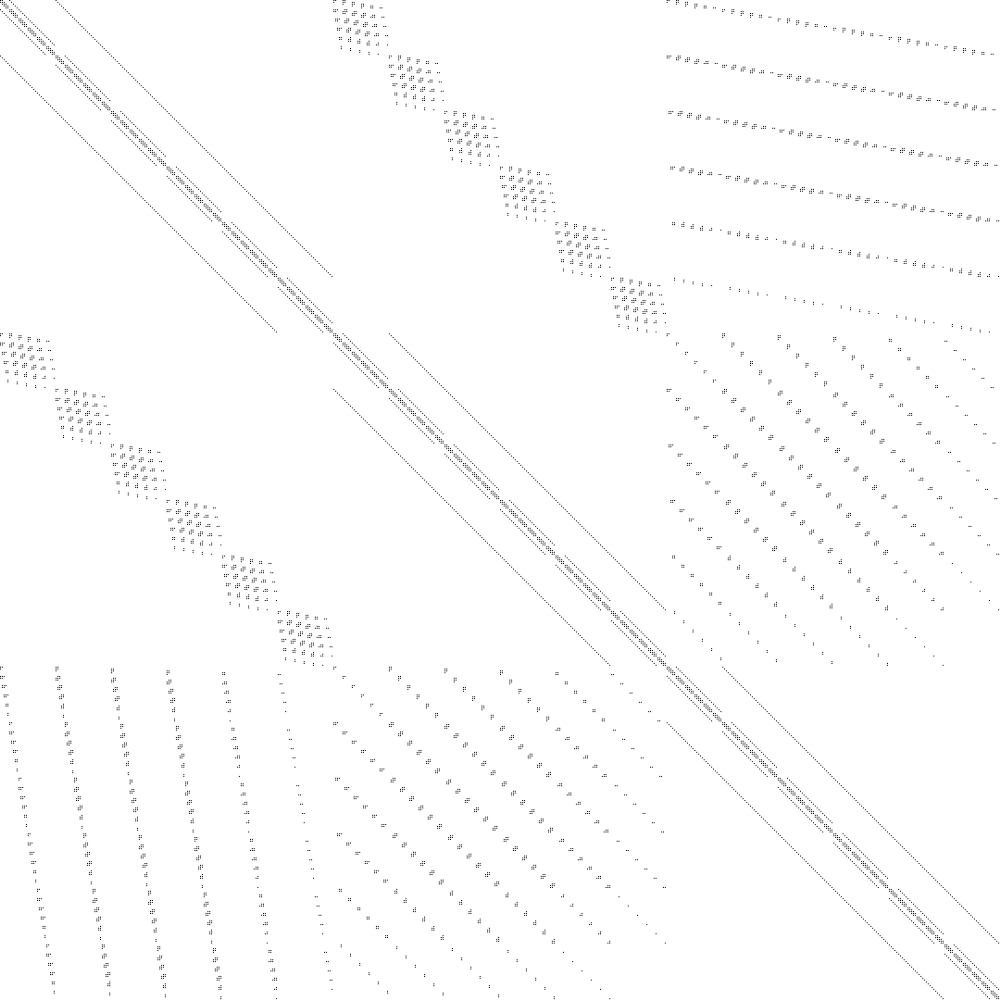
\includegraphics[width=\linewidth]{figures/matrices/m2.pdf}
    \caption{A matrix $M_2$ of size $n=540$ and $8,784$ non-zeroes}
    \label{fig:m2}
\end{figure}

\begin{figure}[h]
    \centering
    \includegraphics[width=\linewidth]{figures/matrices/m3.png}
    \caption{A matrix $M_3$ of size $n=107,811$ and $64,701,513$ non-zeroes}
    \label{fig:m3}
\end{figure}

\end{document}

% Inspired by the International Journal of Computer Applications template
